\chapter{Network Error Logging a relevantné technológie}
\label{nel-and-related-technologies}

Network Error Logging (ďalej už iba \textbf{NEL}) je technológia využívaná vo webovom prostredí, 
kde má svoju rolu v monitorovaní špecifických problémov komunikácie počítačových zariadení využívajúcich služby webu.
Pre dostatočné pochopenie, čím je technológia NEL, v tejto kapitole vysvetľujem najprv 
spomínané prostredie, v ktorom figuruje. 
Následne popíšem, čo predstavujú pojmy monitorovanie a zlyhanie komunikácie na webe, kde zároveň popíšem body, v ktorých môžu rôzne zlyhania nastať. 
V prvom rade sa pri popise problematiky zameriavam na terminológiu, ktorá sa v nadchádzajúcich častiach tejto práce frekventovane používa. 
Samotný popis pre NEL nasleduje za úvodom do technológie, ktorá NEL spojazdňuje ako jeho závislosť, \textbf{Reporting API}, bez ktorej samostatne nemôže \mbox{fungovať \cite{W3C-NEL}}.


\section{Webové prostredie}
\label{webove-prostredie}

V rámci internetu, globálnej infraštruktúry sieťou prepojených zariadení, existuje systém World Wide Web (ďalej už iba web).
Web je služba ponúkajúca možnosť získavať dokumenty uložené na internete, a teda na zariadeniach do neho pripojených, nazývaných taktiež \textbf{web server} \cite{wiki-web}. 
Vyhľadávanie a získavanie spomínaných dokumentov, a teda obsahu dostupného na web serveri, funguje na základe ich vzájomného prepojenia takzvanými hyperlinkami.
Termín \textbf{hyperlink} v tomto kontexte prestavuje taký odkaz na dokument, ktorý umožňuje tento dokument identifikovať, lokalizovať a získať z webu. 
Hyperlinky sa vyskytujú ako súčasti obsahu získavaného dokumentu, a to vo forme či už textu alebo iných médií, ako napríklad obrázkov \cite{wiki-hyperlink}. 


\begin{figure}[htb]
\begin{center}
 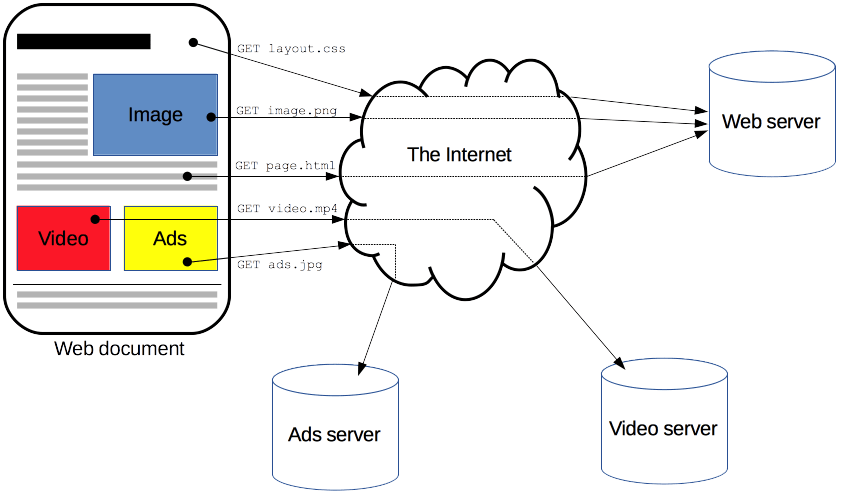
\includegraphics[scale=0.55]{obrazky-figures/fetching_a_page.png}
 \caption{Vizualizácia konceptu webového prostredia. Obrázok prevzatý z \cite{mdn-docs-http-overview}.}
 \label{img:fetching-a-page}
\end{center}
\end{figure}


\pagebreak

\subsection{Štruktúra hyperlinku}
\label{navigacia-na-webe}

Hyperlinky na iné dokumenty sú formované ako reťazcová hodnota nazývaná Uniform Resource Locator \cite{wiki-hyperlink} (jednotný lokátor zdrojov, ďalej už iba \textbf{URL}).
Vďaka hyperlinkom obsahujúcim hodnoty URL je možné odkazovať sa na vzdialený obsah webu, prepájať rôzne dokumenty medzi sebou, a tým web navigovať.
Typická hodnota URL sa skladá z \cite{mdn-docs-url}:
\begin{enumerate}
    \item adresy web servera, teda jeho domény (anglicky \textit{domain}, popísané v sekcii \ref{domeny}),
    
    \item protokolu používaného na sieťovú komunikáciu medzi servermi (anglicky \textit{protocol}),
    
    \item a cesty k uloženému dokumentu (anglicky \textit{path}).
\end{enumerate}

\begin{figure}[htb]
\begin{center}
 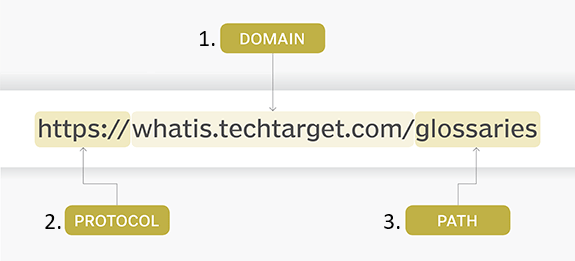
\includegraphics[scale=0.52]{obrazky-figures/the-anatomy-of-a-url.png}
 \caption{Základná štruktúra hodnoty URL. Obrázok prevzatý z internetu.}
 \label{img:urlstructure}
\end{center}
\end{figure}

Tieto hlavné zložky hodnôt URL predstavujú samostatne dôležité koncepty pre navigáciu vo webe.
Podľa príkladu na obrázku \ref{img:urlstructure} prvá časť (1.) označuje doménu web servera, druhá (2.) komunikačný protokol a tretia (3.) cestu k dokumentu. 

\pagebreak

Hodnoty bývajú rôzne a môžu sa skladať z niekoľkých ďalších častí, no tie však nie je potrebné pre účely tejto práce rozoberať.
Protokol definuje množinu platných pravidiel pre komunikáciu zariadenia návštevníka webu s web 
serverom, ktorého prislúchajúce meno je definované ďalšou časťou URL --- doménou. 
Cestu k uloženému dokumentu web server použije pre určenie miesta, kde je požadovaný dokument uložený. 
Ak web server vyžiadaný dokument nájde, zašle ho naspäť danému návštevníkovi webu \cite{mdn-docs-url, wiki-web}.
V ďalších sekciách tento proces postupne opisujem detailnejšie.


\subsection{Domény}
\label{domeny}

Pre adresovanie počítačových zariadení na internete sa používa adresa \textbf{IP}.
Takáto adresa môže mať dve podoby \cite{mdn-docs-domain}:
\begin{enumerate}
    \item IPv4, napríklad \code{192.168.1.1},
    \item IPv6, napríklad \code{2400:cb00:2048:1::c629:d7a2}.
\end{enumerate}


Pomocou takýchto adries taktiež funguje navigácia na internete, označovaná pojmom smerovanie správ v komunikácií medzi počítačmi.
Popis funkcionality smerovania správ nie je dôležitý pre oblasť záujmu tejto práce, no dôležitým faktom je, 
že smerovanie dokumentov vo webovom prostredí funguje na základe smerovania správ pomocou IP adries.

Ďalej sa využíva protokol TCP, ktorého úlohou je nadviazať spojenie medzi dvoma počítačmi označenými adresami IP.
Využitie týchto dvoch hlavných a niekoľko ďalších protokolov v spojení sa označuje za TCP/IP sieťovú komunikáciu \cite{wiki-tcpip}.

Vo webovom prostredí však prenášané dokumenty môžu byť uložené na nespočetne veľkom počte počítačových zariadení.
Dôležitou skutočnosťou je, že IP adresa web serveru poskytujúceho nejaký dokument sa môže časom meniť.
Ďalej, pre návštevníkov webu je nepraktické pamätať si zložité IP adresy pre dokumenty, ktoré chcú vyhľadať.
Z týchto dôvodov sa zaviedlo používanie \textbf{doménových mien}, ktoré predstavujú mená priradené adresám IP v systéme nazvanom 
Domain Name System (\textbf{DNS}, systém doménových mien), ktorý ich spravuje. 
Využitím systému DNS je teda možné v hodnotách URL namiesto zložitých cieľových IP adries používať doménové mená k nim priradené \cite{cloudflare-dns}. 

\subsubsection{Systém doménových mien}

DNS je distribuovaný systém doménových mien prislúchajúcich k IP adresám počítačových zariadení na internete.
Na skladovanie a spravovanie týchto mapovaní používa DNS špecifické databáze pre svoj systém. 
Jeho primárnou službou je vyhľadávanie IP adries podľa spomínaných doménových mien.
Táto služba sa nazýva \textbf{DNS rezolúcia} (anglicizmus, pojem sa do slovenčiny doslovne neprekladá). 
O vykonávanie rezolúcií sa stará program nazvaný \textbf{DNS rezolver} \cite{cloudflare-dns} (tiež anglicizmus použitý pre zachovanie terminológie z čerpaných zdrojov).
Proces pridania IP adresy do systému DNS \mbox{s jej} novým doménovým menom sa nazýva \textbf{registrácia}.


\subsubsection{Štruktúra doménového mena}

Ako bolo zmienené, doménové meno je textová hodnota reprezentujúca adresu webového serveru.
Doménové meno sa rozdeľuje na viaceré úrovne nazývané levely. 
Jednotlivé levely sú v ňom oddelené znakmi bodky. 
Level na konci (najviac vpravo) v doménovom mene sa nazýva \mbox{\textbf{TLD} -- Top Level Doména}. 

\pagebreak

Ďalší level smerom doľava (predposledná hodnota) sa nazýva \textbf{SLD} -- Second Level Doména.
Každý nasledovný level jednak predstavuje level vyššieho rádu (napríklad Third Level Doména, píše sa 3LD) a taktiež je takzvanou \textbf{subdoménou} pre levely nasledujúce za ňou -- v prípade 3LD sú to levely SLD a TLD.

V doménovom mene \code{example.domain.com} platí rozdelenie nasledovne \cite{michal-spacek-etld-article}: 
\begin{itemize}    
    \item \code{\underline{com}}: TLD,
    \item \code{\underline{domain}.com}: podčiarknuté je SLD, spolu levely tvoria názov registrovanej domény,
    \item \code{\underline{example}.domain.com}: podčiarknuté je 3LD, spolu levely tvoria názov subdomény.
\end{itemize}

Okrem jednoduchého rozdelenia na levely sa tiež hodnoty doménového mena oddelené bodkou radia podľa ich logického významu na registrovateľnú doménu a efektívnu TLD.
Túto skutočnosť popisuje nasledujúci \mbox{obrázok \ref{fig:domain-name-structure}}, \mbox{ktorý} berie v úvahu doménové meno skladajúce sa až z piatich bodkou oddelených častí.

\begin{figure}[htb]
\begin{center}
 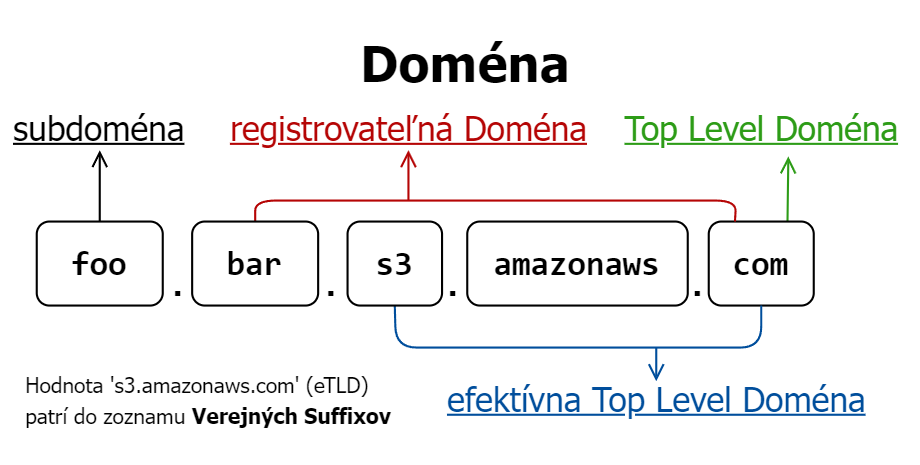
\includegraphics[scale=0.45]{obrazky-figures/domain_name_structure.png}
 \caption{Príklad rozdelenia doménového mena na efektívnu Top Level Doménu a registrovateľnú doménu.}
 \label{fig:domain-name-structure}
\end{center}
\end{figure}


\subsubsection{Verejný Suffix a eTLD}
\label{public-suffix-and-etld}

Doménové meno popisované obrázkom \ref{fig:domain-name-structure} --- \code{foo.bar.s3.amazonaws.com} --- sa ako každé iné doménové meno skladá z TLD, SLD a subdomény. 
Platia tu však niektoré ďalšie dôležité pravidlá pri ich identifikovaní.

Hodnoty TLD môžu byť zložené z viacerých bodkou oddelených hodnôt, pričom stále spolu figurujú ako jeden level.
Doteraz však neexistuje algoritmus pre vyhľadávanie levelu, ktorý by mohol slúžiť na registrovanie domén pre dané zložené TLD -- levelu registrovateľnej domény \cite{mozilla-psl-learn}.
Preto vznikol zoznam nazývaný \textbf{Public Suffix List} (zoznam verejných sufixov, skratka \textbf{PSL}) ako zoznam práve takých TLD, pod ktorými je možné doménu zaregistrovať.
Tieto zložené TLD sa formálne nazývajú efektívne Top Level Domény (\textbf{eTLD}).
Hodnoty eTLD zahŕňajú bežnú hodnotu TLD ako ich poslednú, bodkou oddelenú hodnotu.

\pagebreak

\noindent Preto je pri celých menách registrovaných domén vhodnejšie rozdeľovať ich na eTLD, SLD (meno registrovanej domény) a subdoménu.

S použitím hodnoty eTLD '\code{s3.amazonaws.com}' vybranej z PSL je možné rozdeliť doménové meno z obrázka \ref{fig:domain-name-structure} na jeho levely nasledovne \cite{michal-spacek-etld-article}: 
\begin{itemize}
    \item \code{s3.amazonaws.com}: eTLD, kde \code{.com} je TLD,
    \item \code{bar.s3.amazonaws.com}: celé meno SLD -- registrovanú doménu,
    \item \code{foo.bar.s3.amazonaws.com}: celé meno subdomény.
\end{itemize}

Na záver chcem ako poznámku uviesť, že sa môže pre označenie domény registrovateľnej pod eTLD vyskytovať aj výraz rovnakého významu 
-- \textit{Pay Level Domain} (PLD, preložiteľné so zachovaním významu ako doména zakúpiteľného levelu).
Keďže pojem registrovateľná doména a skratka PLD sú zameniteľné, no PLD sa zväčša v literatúre nepoužíva, 
ďalej \mbox{v práci} domény tohto typu označujem pomocou pojmu registrovateľná doména.


\subsection{Protokol HTTP}
\label{protokol-http}

V oblasti sietí termín protokol predstavuje štandardizovanú množinu pravidiel pre vzájomnú komunikáciu medzi počítačovými zariadeniami \cite{cloudflare-protocol}.
Vzhľadom na to, že funkčnosť technológie NEL sa zakladá na komunikácií za pomoci protokolu HTTPS  \cite{nel-client-side-measurement-e2e-reliability},
venujem sa v tejto sekcii výhradne protokolom HTTP a jeho zabezpečenej verzii, ktorou je práve spomínaný HTTPS.

HTTP, celým názvom HyperText Transfer Protokol, je bez stavový aplikačný protokol pre distribuované hypertextové informačné systémy \cite{rfc9110}. 
Poskytuje jednotné komunikačné rozhranie pre prenos dokumentov (ďalej v terminológií špecifikácie HTTP už iba ako \textbf{zdroj}).
Toto rozhranie definuje dva typy zasielateľných správ --- \textbf{žiadosť} a \textbf{odpoveď}. 
Žiadosť predstavuje doslova žiadosť o zdroj. 
Odpoveď je reakciou na žiadosť, kde je možné, že sa navráti buď žiadaný zdroj, alebo popis chyby, ktorá vznikla pri pokuse o jeho \mbox{navrátenie \cite{rfc7230}}. 

Protokol funguje na základe klient-server komunikácie. Klient zasiela požiadavku na server a server mu naspäť posiela odpoveď.
Koncept takejto komunikácie je znázornený na obrázku \ref{fig:http-client-server}.

\begin{figure}[htb]
\begin{center}
    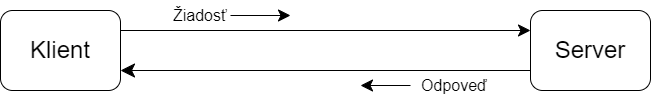
\includegraphics[scale=0.6]{obrazky-figures/http-client-server.png}
    \caption{Znázornenie komunikácie klient-server.}
    \label{fig:http-client-server}
\end{center}
\end{figure}

Klient a server sú názvy rolí, ktoré môžu prepojené zariadenia zaujať v rámci komunikácie pomocou HTTP:
\begin{itemize}
    \item \textbf{Klient} zakladá spojenie so serverom za účelom zasielania jednej alebo viacerých \mbox{žiadostí}: 
    
    Program implementujúci komunikačné rozhranie pre rolu klienta sa nazýva tiež \textbf{User Agent} \cite{rfc9110} (skrátene UA, slovensky -- agent používateľa). 
    Pre bežného návštevníka webu ako UA \mbox{figuruje} \textbf{webový prehliadač} nainštalovaný na jeho zariadení. 
    Webovým prehliadačom sa viac venuje sekcia \ref{webovy-prehliadac}.
    
    \item \textbf{Server} prijíma spojenia aby obslúžil žiadosti tým, že na ne zasiela prislúchajúce odpovede:

    Pre program implementujúci rozhranie takéhoto servera sa používa označenie \textbf{Origin Server} (server pôvodu zdroja, ďalej ako \textbf{origin}).
\end{itemize}


\subsubsection{HTTP žiadosť}

Správy HTTP protokolu sú štruktúrované bloky textu.
Správa nadväzujúca HTTP spojenie, teda žiadosť, má nasledovný obsah \cite{rfc7230, mdn-docs-http-overview}:
\begin{enumerate}
    \item Metóda žiadosti:

    Metóda žiadosti indikuje operáciu, ktorú klient chce aplikovať na žiadaný zdroj.
    Podľa metódy server zistí, aký výsledok úspešne aplikovanej operácie očakáva klient v odpovedi.

    Dôležité metódy sú najmä \cite{rfc9110}:
    \begin{itemize}
        \item GET --- klient žiada zdroj v jeho aktuálnom stave. 
        \item POST --- klient chce vykonať špecifický proces s obsahom, ktorý pridá k žiadosti. 
        Bežne sa jedná napríklad o nahranie nového zdroju z klienta na server.
    \end{itemize}
    
    \item Cesta k požadovanému zdroju:

    Jedná sa tu o cestu spomínanú v sekcii \ref{navigacia-na-webe}, bod 3. v popise príkladnej URL (viď obrázok \ref{img:urlstructure}).
    Cesta môže byť symbolická, teda určená pre interpretáciu samotným serverom (podľa jeho konfigurácie) ako napríklad \code{/glossaries}, alebo priamo označujúca konkrétny zdroj, napríklad \code{/glossaries.txt}.
 
    \item Verzia protokolu HTTP použitého na nadviazanie a priebeh komunikácie.
    
    \item Sekcia polí s ďalšími informáciami a nastaveniami komunikácie -- \textbf{HTTP Headers}:
    
    Táto hovorovo nazývaná sekcia \textbf{hlavičiek} obsahuje páry názvov polí a ich priradených hodnôt. 
    Hlavičky slúžia ako definície možností a iných potrebných informácií pri komunikácií medzi zariadeniami.
    Pre názvy hlavičiek existuje register \textit{Hypertext Transfer Protocol (HTTP) Field Name Registry} \cite{rfc9110},
    v ktorom sa uvádzajú oficiálne hlavičky použiteľné pri komunikácií HTTP. 

    Príkladom potrebnej informácie pre HTTP žiadosť je hlavička \code{Host}, ktorej hodnota musí reprezentovať doménu cieľového web servera. 
    
    \item Prípadný obsah žiadosti:

    Napríklad obsah pridaný k žiadosti s metódou POST. 
    Obsah sa pridáva pod sekciu HTTP hlavičiek, od ktorej sa oddeľuje prázdnym riadkom (znakmi \code{\textbackslash r\textbackslash n}).

    \item Zakončenie správy: dva prázdne riadky (znaky \code{\textbackslash r\textbackslash n\textbackslash r\textbackslash n}).

\end{enumerate}

\begin{figure}[htb!]
\begin{center}
    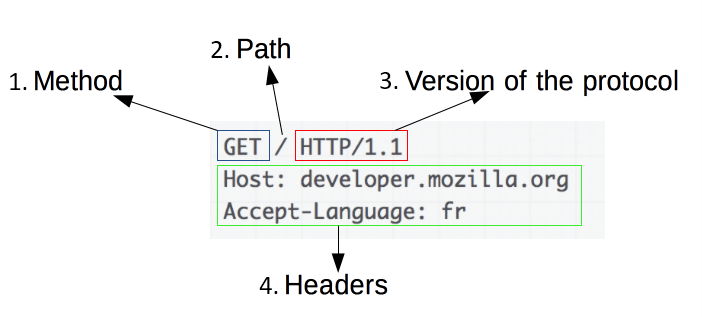
\includegraphics[scale=0.6]{obrazky-figures/http_request.png}
    \caption{Príklad obsahu HTTP žiadosti. Obrázok prevzatý z \cite{mdn-docs-http-overview}.}
    \label{fig:http-request}
\end{center}
\end{figure}

Jednotlivé časti žiadosti sú zobrazené na obrázku \ref{fig:http-request} a označené číslami. Postupne, prvá časť (1.) predstavuje metódu žiadosti, nasleduje cesta \mbox{k zdroju (2.)}. 
Ďalšia je vyznačená verzia protokolu HTTP (3.), pod ktorou je v poslednom rade umiestnená sekcia \mbox{s HTTP} hlavičkami (4.) 


\subsubsection{HTTP odpoveď}

\noindent HTTP odpoveď sa od žiadosti mierne líši. Obsahuje nasledovné časti \cite{rfc7230, mdn-docs-http-overview}:

\begin{enumerate}
    \item Verzia protokolu HTTP použitého na odoslanie odpovede.

    \item Statusový kód reprezentujúci výsledok operácie vyvolanej HTTP žiadosťou:

    Takýto kód v je v odpovedi reprezentovaný ako trojciferné celé číslo, ktoré môže popisovať jeden
    zo stavov rozdelených do piatich kategórií podľa ich významu. 
    Kategórie významov sú určené prvou číslicou čísla statusového kódu, ktoré môže nadobúdať hodnoty od 1 po 5:

    \begin{enumerate}
        \item 1xx (informácia),
        
        % Status tohto typu s hodnotami od 100 do 199 indikuje predbežné odpovede určené pre komunikáciu stavu pripojenia (v komunikácií HTTP) alebo stavu priebehu spracovania prislúchajúcej žiadosti.
        % Odpovede so statusom 1xx sa zasielajú predtým ako sa dokončí operácia vyžiadaná žiadosťou a zašle sa pre ňu finálna odpoveď.
        
        \item 2xx (úspech),
        
        % Statusy 2xx s hodnotami od 200 do 299 oznamujú klientovi, že jeho žiadosť bola úspešne prijatá, spracovaná a akceptovaná. 
        
        \item 3xx (presmerovanie),
        
        % Status 3xx indikuje, že pre dokončenie obsluhy žiadosti klienta musí klient vykonať ďalšiu alebo inú akciu.
        % V odpovedi obsahujúcej presmerovanie sa teda nachádza nový zdroj, ktorý by mal klient vyžiadať, aby mohla byť dokončená obsluha jeho pôvodnej žiadosti. 
        % Statusy tejto kategórie môžu nadobúdať hodnoty od 300 do 399.
        
        \item 4xx (chyba klienta),

        % Status chyby klienta s hodnotami od 400 do 499 oznamuje klientovi, že sa vyskytol problém s jeho žiadosťou.
        % Server teda zasiela klientovi odpoveď, v ktorej vysvetľuje chybu v jeho žiadosti.
        
        \item 5xx (chyba servera).

        % Hodnoty 500 až 599 označujú problémy, ktoré vznikli na strane servera jeho vlastným zapríčinením, alebo zapríčinením jeho závislostí (databáza, sieťové operácie a podobne).
        % Server, ktorý odošle odpoveď so statusom z tejto kategórie oznamuje klientovi, že jeho žiadosť nemôže byť obslúžená, pretože pri obsluhe server zlyhal.
    \end{enumerate}

    \item Správa prislúchajúca k statusovému kódu:

    Konkrétny význam statusového kódu však dopĺňajú zvyšné dve číslice kategórie, ktoré sú v jednotlivých kategóriách vyššie reprezentované nahraditeľnými znakmi \code{xx}.
    Tieto zvyšné číslice môžu nadobúdať hodnoty od 0 po 99.
    Ku každej takejto hodnote statusového kódu prislúcha nejaká popisná správa sformovaná ako obyčajný reťazec zakončený ASCII znakom pre nový riadok. 
    Správy sú štandardizované ako frázy spísané v anglickom jazyku.
    Medzi najbežnejšie statusové správy podľa statusových kódov patria:

    \begin{itemize}
        \item \code{100} -- \code{CONTINUE}: Server pokračuje v spracovávaní žiadosti,
        \item \code{200} -- \code{OK}: Žiadosť úspešne spracovaná,
        \item \code{301} -- \code{MOVED PERMANENTLY}: Zdroju bola priradená iná URL,
        \item \code{404} -- \code{NOT FOUND}: Zdroj sa nenašiel,
        \item \code{500} -- \code{INTERNAL SERVER ERROR}: Server pri obsluhe žiadosti zlyhal.
    \end{itemize}

    \item Sekcia s hlavičkami:

    Táto sekcia je štruktúrovaná rovnako ako v HTTP žiadosti. V prípade odpovede sem však naviac pribúdajú ďalšie hlavičky, ktoré by odpoveď mala zahŕňať: 

    \begin{itemize}
        \item \code{Date}: dátum a čas odoslania odpovede,
        \item \code{Server}: software nainštalovaný na web serveri (origin server), ktorý odpoveď zaslal,
        \item \code{Content-Length}: dĺžka obsahu odpovede v bajtoch,
        \item \code{Content-Type}: typ média prenášaného v obsahu odpovedi.

        Hodnota typu média musí byť jedným s registrovaných názvov typov v zozname \textit{Multipurpose Internet Mail Extensions} (MIME). 
        Príkladmi MIME typov pre prenášaný obsah sú hodnoty \code{text/plain} pre obyčajný text, \code{text/html} pre HTML alebo \code{image/png} pre obrázky.
    \end{itemize}

    \item Obsah odpovede:

    Pre umiestnenie obsahu v odpovedi platí to isté ako pre obsah umiestnený v žiadosti.
\end{enumerate}

\begin{figure}[htb!]
\begin{center}
    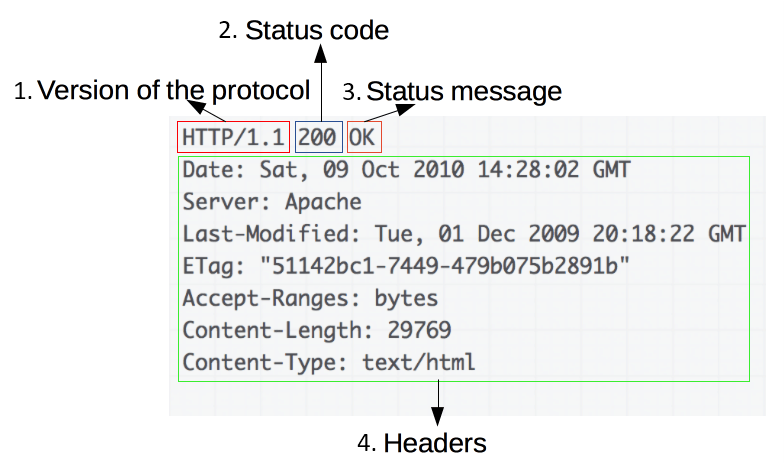
\includegraphics[scale=0.6]{obrazky-figures/http_response.png}
    \caption{Príklad obsahu HTTP odpovede. Obrázok prevzatý z \cite{mdn-docs-http-overview}.}
    \label{fig:http-response}
\end{center}
\end{figure}

Jednotlivé časti odpovede sú zobrazené na obrázku \ref{fig:http-response} a označené číslami. 
Prvú časť (1.) tvorí verzia protokolu HTTP, za ňou sa nachádza \mbox{statusový kód (2.)} a správa k nemu prislúchajúca (3.). 
Pod nimi je na konci odpovede umiestnená sekcia s HTTP hlavičkami (4.). 
Väčšinou býva k odpovedi pridaný aj dodatočný obsah, ktorý by nasledoval ako časť oddelená prázdnym riadkom od hlavičiek.

\pagebreak


\subsubsection{HTTPS}

Dáta spomínané v sekciách o žiadosti a odpovedi sa prenášajú v HTTP komunikácií ako obyčajný text. 
Tým pádom v prípade odpočúvania a potencionálneho pokusu o ovplyvnenie tejto komunikácie má tretia strana (útočník) prístup k všetkým prenášaným dátam. 
To znamená, že útočník následne môže dáta z komunikácie čítať, pozmeniť alebo pridať svoj vlastný obsah. 
Je teda nutné ochrániť komunikáciu klienta so serverom pred nežiadúcimi zásahmi z tretej strany. 
Z toho dôvodu bol vyvinutý protokol HTTPS -- Secure (bezpečný) HTTP.
HTTPS je zabezpečená verzia protokolu HTTP, ktorá šifruje obsah prenášaných správ medzi klientom a serverom.
V kontextoch senzitívnych operácií vykonávaných na webe, ako napríklad prenos súkromných dokumentov, poskytuje HTTPS bezpečný spôsob vymieňania dát so serverom \cite{cloudflare-http-not-secure}.

O samotné šifrovanie v rámci prenosu HTTPS sa stará protokol TLS -- Transport Layer Security (bezpečnosť prepravnej vrstvy).
TLS je rovnako ako HTTP protokol pre komunikáciu klienta so serverom a jeho použitím pri komunikácií HTTP sa spojenie medzi zariadeniami zabezpečuje proti odpočúvaniu, manipulácií a falšovania správ \cite{cloudflare-tls}. 


\subsection{Obsah hľadaných dokumentov}
\label{obsah-hladanych-dokumentov}

Webové dokumenty, alebo iným pomenovaním -- webové zdroje, sa prenášajú v prostredí webu pomocou protokolu HTTP  (viď obrázok \ref{img:fetching-a-page}).
Tieto dokumenty sú buď získané samostatne ako jednotlivé súbory (textový súbor, obrázok, archív \code{.zip}), alebo ako zoskupená množina viacerých súborov v podobe webovej stránky.

Webová stránka (skrátene \textbf{webstránka}) je typ dokumentu, ktorého obsahom je hypertext štruktúrovaný vo formáte \textbf{HTML} \cite{documents-webpage}.
HTML je formát webového dokumentu skladajúceho sa z počiatočnej definície typu dokumentu a stromovej štruktúry takzvaných elementov, kde prvým je element \code{<html>}. 
Jednotlivé elementy sa do HTML súboru vpisujú pomocou značiek, pričom, okrem jednotlivých výnimiek, 
každý element musí mať otváraciu (\code{<elementXY>}) a zatváraciu značku (\code{</elementXY>}).
Vnútorne sa HTML delí na dve hlavné sekcie --- \textbf{hlavičku} pre metadáta dokumentu a \textbf{telo} pre jeho vnútorné rozpoloženie a obsah.
Elementy môžu mať k sebe priradené položky uchovávajúce ich doplnkové detaily nazývané atribúty. 
Napríklad element používaný pre vytvorenie hyperlinku s názvom \code{\textbf{<a>}} (anglicky skratka pre \textit{anchor}) 
môže mať priradený atribút s názvom \code{\textbf{href}} obsahujúci URL odkazovaného dokumentu \cite{documents-html-spec}. 
Vo výpise \ref{listing:html-struktura} ukážka HTML obsahuje počiatočnú definíciu typu dokumentu (\code{<!DOCTYPE html>}), hlavičku, telo, hyperlink a popisné komentáre.


\begin{center}
\centering
\begin{lstlisting}[caption={Príklad základnej štruktúry obsahu HTML dokumentu.},
label=listing:html-struktura, 
language=HTML, 
frame=tb,
xleftmargin=.05\textwidth, 
xrightmargin=.05\textwidth]
    <!DOCTYPE html>
    <!-- %*Toto je komentár, ktorý sa na stránke klientovi nezobrazí*) -->
    <html lang="sk">       
        <!-- %*HTML hlavička*) -->
        <head>
         <title>%*Príklad HTML dokumentu*)</title>
        </head>
        <!-- %*HTML telo*) -->
        <body>
         <!-- %*Ukážka vytvorenia hyperlinku: element <a> a jeho atribút href*) -->
         <a href="https://google.com">%*Hypertext odkazujúci na stránku google*)</a>
        </body>
    </html>
\end{lstlisting}
\end{center}

Vo výpise \ref{listing:html-struktura} súbor HTML však obsahuje odkaz iba na vzdialenú webstránku.
Pridať odkazy na rôzne iné médiá ako obrázky, audio a video (ale aj dokumenty HTML), je však možné vďaka dvom ďalším kategóriám elementov. 
Sú nimi \cite{documents-html-spec}: 
\begin{enumerate}
    \item Elementy \code{<link>} patriace do hlavičky HTML.

    Tieto elementy odkazujú na vzdialené metadáta pre samotnú webstránku.
    Typ metadát udáva atribút s názvom \code{rel}, ktorý môže nadobúdať napríklad hodnotu 
    \code{'author'} alebo \code{'help'} pre vytvorenie odkazu na autora stránky, alebo dokumentu poskytujúcemu 
    pomocný manuál pre obsah stránky.
    
    \item Elementy obsahujúce atribút \code{src} patriace do tela HTML.

    Akýkoľvek element z tejto kategórie môže odkazovať na podporovaný typ média, ktorý udáva názov takéhoto elementu.
    Ide napríklad o elementy: 
    \begin{itemize}
        \item \code{<img>} -- obrázky,
        \item \code{<audio>} -- audio súbory,
        \item \code{<video>} -- videá,
        \item \code{<iframe>} -- HTML dokumenty, ktoré možno vnoriť do inej webstránky.
    \end{itemize}
    
\end{enumerate}

Každé samostatné médium, ktoré tieto elementy označujú je potrebné získať ako zdroj ďalšou HTTP žiadosťou spolu so samotnou webstránkou, ktorá na dané médium odkazuje.

\subsection{Webový prehliadač}
\label{webovy-prehliadac}

% search engine
% http://infolab.stanford.edu/%7Ebackrub/google.html

Softvér slúžiaci pre získavanie zdrojov na webe, stavaný ako implementácia HTTP klienta, teda ako UA (User Agent) sa nazýva webový prehliadač \cite{mdn-docs-browser}. 
Tým, že je prehliadač implementáciou HTTP klienta (viď sekciu \ref{protokol-http}), dokáže zasielať žiadosti a spracovávať odpovede HTTP.
Je to teda program, ktorý využíva koncepty vysvetlené vyššie a je schopný prehľadávať web.

Používateľ s nainštalovaným prehliadačom má teda možnosť vyhľadávať webstránky.
Webstránky sú v prehliadači vybudované a zobrazené podľa ich obsahu HTML (viď sekciu \ref{obsah-hladanych-dokumentov}).
Na uskutočnenie tohto procesu vybudovania a zobrazenia webstránky používa prehliadač svoje zabudované algoritmy \cite{mdn-docs-how-browser-works}.
Moderné webstránky okrem samotného zdroja HTML obsahujú aj prídavné závislé zdroje, ktoré môžu priamo danej webstránke upraviť vzhľad alebo pridať programovateľnú funkcionalitu.
Prehliadač takéto zdroje získava pomocou odkazov, ktoré sú definované v hlavičke alebo tele dokumentu HTML prislúchajúceho danej webstránke.

V tejto práci je dôležité popísať konkrétne zdroje pridávajúce programovateľnú funkcionalitu.
Sú nimi zdroje obsahujúce prehliadačom spúšťateľné skripty napísané v programovacom jazyku JavaScript.

\subsubsection{JavaScript}
\label{javascript}

JavaScript je programovací jazyk, ktorého využitím je v oblasti webu práve robiť webstránky interaktívnymi \cite{mdn-docs-js}. 
Jedným z jeho využití je manipulácia so stromovou štruktúrou obsahu HTML dokumentu (viď sekciu \ref{obsah-hladanych-dokumentov}).
Funkcionalita zabezpečujúca podporu pre takúto manipuláciu s obsahom webstránok a ďalšie podobné funkcionality sú v jazyku JavaScript dostupné ako \textbf{Web API}.

API\footnote{API -- Application Programming Interface (programové rozhranie aplikácie)} predstavuje predprogramovaný balík kódu, ktorý uľahčuje jeho používateľom, teda programátorom, prácu v oblasti zamerania funkcionality daného balíka \cite{mdn-docs-web-api}.
Ďalej, skutočnosť, že ide o webové API znamená, že je možné taký balík využiť prostredníctvom JavaScriptu spojeného s webstránkou.
Existuje množstvo webových API, z ktorých niektoré sú poskytované priamo prehliadačom používateľa webu, iné zasa tvorcami tretej strany (Third-party API).

\subsubsection{JavaScript Object Notation}
\label{json}

V spojení s konceptami jazyka JavaScript vznikol jeden konkrétne dôležitý textový formát dát s názvom \textbf{JSON} -- JavaScript Object Notation \cite{rfc7159}.
Štruktúra formátu JSON je jednoduchá a je založená na niektorých dátových typoch jazyku JavaScript.
Dokáže reprezentovať nasledovné dátové typy:
\begin{enumerate}
    \item primitívne: reťazce, čísla, pravdivostné hodnoty (\code{boolean}) a absenciu hodnoty (\code{null})
    
    \item štruktúrované: 
    \begin{enumerate}
        \item Polia (ďalej ako JSON array):

        Array je usporiadaná sekvencia 0 a viac hodnôt. Označuje sa zátvorkami \code{[} a \code{]}. 

        \item Objekty:

        Objekt je neusporiadaná kolekcia 0 a viac párov kľúč--hodnota, kde kľúč je reťazec
        a hodnota môže byť akýkoľvek primitívny alebo štruktúrovaný dátový typ.
        Označuje sa zátvorkami \code{\{} a \code{\}}.
    \end{enumerate}
\end{enumerate}

JSON má využitie napríklad ako formát dát pri komunikácií typu HTTP na webe.
\mbox{V správach}, ktoré obsahujú zdroj typu JSON musí byť nastavená HTTP hlavička s názvom \code{Content-Type} na hodnotu typu MIME \code{application/json}.

Vo výpise \ref{listing:priklad-dokumentu-json} je uvedený príklad takéhoto dokumentu. Položka \code{"student"} predstavuje JSON kľúč, ktorého hodnotou je štruktúrovaný dátový typ objekt. Názornú ukážku dátového typu pole predstavuje hodnota priradená kľúču \code{"predmety"}.

\begin{center}
\centering
\begin{lstlisting}[
caption={Príklad obsahu dokumentu JSON.},
label=listing:priklad-dokumentu-json, 
language=json, 
frame=tb,
xleftmargin=.15\textwidth, 
xrightmargin=.15\textwidth]
    {       
        "student": {
            "login": "xjurik12",
            "kredity": 162,
            "predmety": ["ITT", "IBP"],
            "vyborny_priemer": false
            "diplom": null
        }
    }
\end{lstlisting}
\end{center}

\pagebreak


\section{Monitorovanie zlyhaní webstránok}

Cieľom tejto práce je analyzovať technológiu spojenú s monitorovaním zlyhaní v komunikácií 
na webe --- Network Error Logging (NEL).
Technológie, na ktorých sa NEL zakladá alebo ich používa, boli vysvetlené v predošlej sekcii \ref{webove-prostredie}.
Ďalej už popisujem termíny spojené priamo s NEL.

\subsection{Monitorovanie}
\label{monitorovanie}

Pojem \textit{monitorovanie webstránok} je na verejne dostupných zdrojoch definovaný ako proces testovania a kontrolovania či používateľ webu, konkrétne danej webstránky, môže s ňou pracovať tak, ako to očakáva jej poskytovateľ \cite{wiki-website-monitoring}. 
Webstránku však možno zameniť za akýkoľvek zdroj uložený na webe.
Správca webového serveru, kde sa zdroj nachádza, môže používať monitorovanie pre získanie informácií ohľadom zlyhaní pri jeho dopyte.
Monitorovacie nástroje zaznamenávajú žiadosti o získanie určitého zdroja a na zistené zlyhania upozorňuje správcov zaňho zodpovedných.  
Vďaka aplikovanému monitorovaniu teda správca web serveru nadobúda prehľad o stave dostupnosti ním spravovaných zdrojov a je mu tak umožnené vzniknuté problémy rýchlejšie napraviť.

\subsection{Body zlyhania}
\label{body-zlyhania}

Proces prehliadania webu možno definovať ako získavanie vzdialených zdrojov, napríklad webstránok, použitím webového prehliadača.
Za predpokladu, že používateľ má dostupnú adresu URL pre zdroj (viď sekciu \ref{navigacia-na-webe}), 
ktorý chce získať, má tento proces nasledovnú postupnosť úkonov na vykonanie \cite{nel-client-side-measurement-e2e-reliability, mdn-docs-how-browser-works}:

\begin{enumerate}
    \item prehliadač získa adresu IP pre doménu web serveru z danej URL v systéme DNS,
    
    \item prehliadač vytvorí so zariadením adresovaným získanou IP adresou spojenie protokolom TCP,
    
    \item prehliadač použije spojenie TCP s web serverom na zasielanie HTTP žiadostí 
    (popísaných v sekcii \ref{protokol-http}) s cieľom získať zdroj uvedený v danej URL.
\end{enumerate}

Každý z vyššie uvedených krokov môže skončiť s nejakou chybou, čo by spôsobilo celkové zlyhanie procesu získania cieľového zdroja.
Na základe týchto troch potrebných krokov pre úspešné získanie zdroja možno rozdeliť zlyhania do troch kategórií \cite{nel-client-side-measurement-e2e-reliability, W3C-NEL}:
\begin{enumerate}
    \item Zlyhania komunikácie s DNS:

    Tieto zlyhania môžu zahŕňať nedostupnosť DNS servera, chybové odpovede bez nájdenej 
    IP adresy web servera so zdrojom alebo iné neočakávané zlyhania ako napríklad náhle prerušenie spojenia s DNS serverom.
    
    \item Zlyhania nadviazania spojenia TCP/IP:

    Spojenie s webovým serverom, na ktorom je zdroj uložený, môže zlyhať pri:
    \begin{itemize}
        \item Zakladaní spojenia.
        
        Adresa IP servera je neplatná, server je nedostupný alebo spojenie neprijal.
        
        \item Náhlom ukončení spojenia.

        Server môže spojenie uzavrieť, resetovať, alebo skrátka prerušiť.  

        \item Alebo pri zakladaní bezpečného spojenia.

        Komunikácia pomocou zabezpečeného protokolu HTTPS, ako už bolo spomínané, využíva na zabezpečenie základnej verzie HTTP protokol nazvaný TLS.
        TLS spojenie sa vytvorí, iba ak sú pre také spojenie splnené požiadavky na ako webového klienta, tak aj webový server. 
        Zlyhania zakladania TLS spojenia môžu nastať pri rôznych prípadoch nesplnenia týchto požiadaviek.

    \end{itemize}
    
    \item Zlyhania prenosu HTTP:

    \begin{enumerate}
        \item Zlyhanie samotného protokolu.

        Napríklad môže programovo zlyhať softvér pre HTTP origin server (chyba v implementácií origin servera).
        HTTP odpoveď môže byť nesprávne skonštruovaná, napríklad, keď obsahuje konfliktné hodnoty hlavičiek a obsahu (hodnota hlavičky \code{Content-Length} nesedí so skutočnou dĺžkou obsahu).  
        Ešte však dochádza aj \mbox{k situáciám}, pri ktorých sa vytvorí takzvaný \textit{redirect loop}, čo predstavuje slučku presmerovaní HTTP klienta. Takáto slučka spôsobuje, že klient neustále zasiela tú istú sekvenciu žiadostí, no nikdy sa nedopracuje k cieľovému zdroju.
        
        \item HTTP odpoveď navrátená so statusom z kategórie 4xx alebo 5xx.

        Odpovede so statusom 5xx reprezentujú zlyhanie na strane origin servera, ktorý nebol schopný poskytnúť vyžiadaný zdroj.
        Naopak, odpovede so statusom 4xx sú chybami na strane klienta. 
        Avšak, aj tieto chyby sú z hľadiska monitorovania vzácne, pretože nadmerne časté opakovanie takejto chyby môže pomôcť odhaliť nesprávne zadefinované (alebo jednoducho zastarané a neudržované -- status 404) hyperlinky na webstránke správcu, ktorý ju monitoruje. 
    \end{enumerate}
    
\end{enumerate}


\section{Network Error Logging}
\label{network-error-logging}

Podľa definície monitorovania zo sekcie \ref{monitorovanie}, NEL slúži ako mechanizmus
zabezpečujúci monitorovanie zlyhaní žiadostí pre zdroje uložené na web serveri, ktorý NEL používa \cite{W3C-NEL}.
Autormi NEL sú členovia organizácie World Wide Web Consortium\footnote{\url{https://www.w3.org/about/}}, ktorí pre túto technológiu publikovali špecifikáciu 25. septembra 2018.
Nie je to prvá publikovaná špecifikácia pre túto technológiu.
Avšak je to prvá publikácia, ktorá špecifikuje verziu NEL stabilne používanú do súčasnosti.
V tejto práci vychádzam z najaktuálnejšej dostupnej špecifikácie NEL, publikovanej 5. októbra 2023.
Predtým však, ako sa dostanem k popisu NEL, jeho možnostiam a konfigurácii, musím popísať konkrétnu Web API -- Reporting API, na ktorej je z hľadiska svojej funkcionality závislý.

\subsection{Závislosť na Reporting API}
\label{reporting-api}

Reporting API je jedným z balíkov označovaných názvom Web API (viď sekciu \ref{javascript}).
Serverom, ktoré Reporting API používajú, poskytuje možnosť definovať pravidlá pre 
tvorbu a zasielanie takzvaných hlásení na pravidlami definované web servery.
Hlásenia sa týkajú špecifických záležitostí prehliadača klienta, ktorý žiada zdroje z web serveru používajúceho Reporting API.
Medzi takéto špecifické funkcie patrí práve NEL, ale napríklad aj detegovanie výskytov zlyhaní alebo používania zastaraných API na klientskom prehliadači \cite{W3C-reporting-api}.

Aby bolo možné tento balík uplatniť, musí ho podporovať webový prehliadač (konkrétne User Agent) používateľa, ktorý zasiela žiadosti o získanie zdrojov zo servera využívajúceho Reporting API.

\subsubsection{Verzia používaná technológiou NEL}

Je dôležité podotknúť, že najnovšia verzia tejto API, popísaná špecifikáciou z 10. novembra 2023, nie je kompatibilná s momentálnou technológiou NEL.
Dôvodom je, že technológia NEL je stále v procese vývoja a jej momentálna verzia je implementovaná tak, aby fungovala so staršou verziou Reporting API.
Konkrétne, NEL je kompatibilný s verziou popisovanou v špecifikácií zverejnenej 
25. septembra 2018, taktiež označovanou ako verzia \textbf{\code{v0}}.
Ďalej teda opisujem výhradne Reporting API verzie \code{v0}\footnote{\url{https://developer.chrome.com/blog/reporting-api-migration} (zmienky verzií NEL a Reporting API)}.

\subsubsection{Definícia pravidiel}

Vyššie spomínané pravidlá môže definovať server, ktorý chce využívať tento API balík. 
Definícia pravidiel funguje prostredníctvom zaslania HTTP hlavičky \code{Report-To} v HTTP odpovedi pre vybraný zdroj.
Obsahom hlavičky \code{Report-To} musí byť textová hodnota vo formáte JSON (viď sekciu \ref{json}), pričom jej štruktúru tvorí striktne JSON array objektov.

Špecifickým rozdielom od klasického JSON formátu však je, že sa táto hodnota do hlavičky
zapisuje bez zátvoriek, ktoré bežne tvoria JSON array (znaky '\code{[}' a '\code{]}').
S touto odchýlkou od bežného JSON formátu môže User Agent pracovať vďaka tomu, že pre takto špecifický formát existuje samostatný typ MIME s názvom \code{application/reports+json}. 

Každý objekt v poli hodnôt hlavičky \code{Report-To} predstavuje pravidlo Reporting API.
Pravidlá sa musia ukladať v pamäti User Agenta, ktorému je odpoveď s pravidlami zaslaná.
Hodnota každého pravidla obsahuje nasledovné polia \cite{W3C-reporting-api}: 

\begin{enumerate}

    \item \code{group},

    Pole obsahujúce textový názov skupiny web serverov prislúchajúcich k danému pravidlu.
    
    Ak pravidlo neobsahuje toto pole, názov jeho skupiny web serverov bude \code{"default"}.
    
    \item \code{endpoints},

    Povinné pole \code{endpoints} musí definovať zoznam web serverov, ktoré patria do skupiny definovanou poľom \code{group}.
    
    Každý web server tu predstavuje takzvaný \textbf{kolektor} chybových hlásení.
    Ďalej, pojem \textbf{poskytovateľ kolektorov} predstavuje spoločnú registrovateľnú doménu pre kolektory, ktorých doménové meno je jej subdoménou.
    Napríklad, doména \code{report-uri.com} figuruje ako poskytovateľ kolektorov \code{abc.report-uri.com} aj \code{xyz.report-uri.com}.
    
    Hodnota tohto poľa musí byť JSON array objektov s nasledovným obsahom:
    \begin{enumerate}
        \item \code{url} -- URL adresa kolektora (povinná hodnota).
        \item \code{priority} -- Číslo definujúce prioritu kolektora v rámci skupiny \code{group}.

        Priorita kolektora predstavuje jeho prednosť pred ostatnými v procese výberu kolektora, ktorému bude odoslané vygenerované hlásenie.
        
        \item \code{weight} -- Číslo určujúce prioritu kolektorov s rovnakou hodnotou poľa \code{priority}.

        Tu priorita zase predstavuje prednosť kolektora pred ostatnými pri nerozhodnosti v prípade, že majú viaceré kolektory priradené rovnakú hodnotu \code{priority}.
    \end{enumerate}
    
    \item \code{max\_age},

    Ďalšie povinné pole definujúce životnosť daného pravidla. Jeho hodnotou musí byť nezáporné číslo reprezentujúce sekundy.

    Špeciálnym prípadom hodnoty tohto poľa je číslo \code{0}. 
    V prípade, že server pre pravidlo prislúchajúce konkrétnej skupine \code{group} vyplní \code{max\_age} hodnotou \code{0}, pravidlo stráca platnosť a musí byť vymazané.
    
    \item \code{include\_subdomains}.

    Toto pole obsahuje pravdivostnú hodnotu \code{true} alebo \code{false}.
    Podľa nej web server zasielajúci pravidlo určuje či sa dané pravidlo má používať aj pre subdomény daného web servera.
    Toto pravidlo platí vždy pre jeho skupinu definovanú poľom \code{group}.

    Ak pole nie je uvedené, pravidlo pre skupinu \code{group} sa na subdomény vzťahovať nebude.
    
\end{enumerate}

Výpis \ref{listing:priklad-report-to} obsahuje príklad pravidla Reporting API definovaného v HTTP hlavičke \code{Report-To}. 
Pravidlo tu definuje skupinu s názvom \code{reporting-skupina}, ku ktorej prislúchajú dva kolektory, kam môžu byť hlásenia zasielané s rozdielnou prioritou. 
Doba platnosti pravidla je 2 592 000 sekúnd, teda 30 dní.

\begin{center}
\centering
\begin{lstlisting}[
caption={Príklad obsahu hlavičky \code{Report-To}.},
label=listing:priklad-report-to, 
language=json, 
frame=tb,
xleftmargin=.04\textwidth, 
xrightmargin=.04\textwidth]
    Report-To: {
        "group": "reporting-skupina",
        "endpoints": [
            {"url": "https://example.com/reporting1", "priority": 1},
            {"url": "https://example.com/reporting2", "priority": 2}
        ],
        "max_age": 2592000
    }
\end{lstlisting}
\end{center}


\subsubsection{Tvorba hlásení}

Počas doby platnosti aspoň jedného pravidla Reporting API existujúceho v pamäti 
User Agenta sa na ňom tvoria už spomínané hlásenia.
Hlásenie je správa týkajúca sa jednej \mbox{z hlásiteľných} udalostí, ktoré môžu nastať v prostredí prehliadača implementujúceho daný User Agent.
Medzi tieto hlásiteľné udalosti patrí \cite{W3C-reporting-api}: 
\begin{itemize}
    \item prehliadač použil Web API, ktorá bola označená ako zastaraná,
    \item User Agent zabudovaný v prehliadači sa rozhodol nezaslať ďalšiu HTTP žiadosť na Origin Server z bezpečnostných dôvodov,
    \item prehliadač zlyhal a bol terminovaný,
    \item došlo k zlyhaniu týkajúceho sa oblasti monitorovania NEL.
\end{itemize}


\subsubsection{Zasielanie hlásení}

Nahromadené hlásenia sa periodicky odosielajú na web server cieľovej skupiny \code{group} pravidla vybraný podľa jeho priority.
Špecifikácia verzie \code{v0} Reporting API nedefinuje túto periódu odosielania sama, ale prenecháva túto zodpovednosť na prehliadače, ktoré sa rozhodnú API podporovať \cite{W3C-reporting-api}.

Ďalej, skupín \code{group} je práve toľko, koľko existuje uložených pravidiel s definovaným menom so zarátaním prípadnej skupiny \code{"default"}.
Výber cieľovej skupiny spočíva v ďalšom nastavení súvisiacim s Reporting API --- priradenie typu hlásenia k skupine.
Pre rôzne typy hlásení sa toto nastavenie zavádza inak.
V prípade hlásenia zlyhania v oblasti monitorovania NEL sa skupina \code{group} vyberá v samotnom nastavení pre NEL, ktoré priamo spolupracuje s pravidlami Reporting API.
Tento proces je popísaný v samostatnej špecifikácií NEL, spísanej v sekcii \ref{network-error-logging-spec}.

Hlásenia sa hromadia a čakajú na odoslanie.
Každé z nich sa odošle vo formáte JSON na vybraný kolektor s najvyššou vypočítanou prioritou v nasledujúcej štruktúre:
\begin{itemize}
    \item \code{type} -- typ hlásenia,

    Hodnoty môžu byť napríklad \code{"crash"} alebo \code{"network-error"}.
    
    \item \code{age} -- vek hlásenia,

    Vek hlásenia je čas v milisekundách, ktorý uplynul od jeho vytvorenia webovým prehliadačom.
    Podľa implementácie podpory pre Reporting API môže webový prehliadač nechať nahromadiť viaceré hlásenia a zasielať ich oneskorene.
    
    \item \code{url} -- hodnota URL adresujúcej zdroj pre ktorý sa hlásenie vygenerovalo,
    
    \item \code{user\_agent} -- názov a informácie o User Agentovi webového prehliadača používateľa,
    
    \item \code{body} -- telo hlásenia

    Telo hlásenia je vyplnené pre každý typ hlásenia inak. 
    Príklad jednoduchého hlásenia je vo výpise \ref{listing:priklad-generated-report}.
    Toto hlásenie bolo odoslané 42 milisekúnd po jeho vytvorení na prehliadači Mozilla. Vygenerované bolo chybou, ktorá nastala po získaní zdroja prislúchajúceho k URL \code{https://example.com}. \mbox{Telo hlásenia} obsahuje ID zlyhania a ako dôvod je uvedená hodnota \code{oom}, ktorá reprezentuje chybu \textit{Out Of Memory} (nedostatok pamäte).
    V sekcii \ref{network-error-logging-spec} je uvedený príklad hlásenia typu NEL vo výpise \ref{listing:priklad-nel-report}.
\end{itemize}


\begin{center}
\centering
\begin{lstlisting}[
caption={Príklad obsahu zaslaného hlásenia pre zlyhanie webového prehliadača. Obsah výpisu prevzatý z \cite{W3C-reporting-api}.},
label=listing:priklad-generated-report, 
language=json, 
frame=tb,
xleftmargin=.085\textwidth, 
xrightmargin=.085\textwidth]
{
  "type": "crash",
  "age": 42,
  "url": "https://example.com/",
  "user_agent": "Mozilla/5.0 (X11; Linux x86_64; rv:60.0) Gecko/20100101 Firefox/60.0",
  "body": {
    "crashId": "30437694edfeae5b",
    "reason": "oom"
  }
}
\end{lstlisting}
\end{center}



\subsection{Využitie NEL}
\label{network-error-logging-spec}

NEL, podobne ako Reporting API, je mechanizmus spúšťaný tým, že je klientovi pri žiadosti o cieľový zdroj z monitorovaného web serveru v HTTP odpovedi zaslaná hlavička \mbox{\code{NEL} \cite{W3C-NEL}}.
Hlavička \code{NEL} môže obsahovať jedno alebo viaceré pravidlá určené pre klienta, ktorý ak NEL podporuje, vyberie \textit{prvé} správne sformované pravidlo v poradí a uloží si ho ako \textbf{konfiguráciu} NEL.
Ostatné pravidlá musí User Agent podľa špecifikácie ignorovať.

Spolu s uvedenou hlavičkou s obsahom predstavujúcim konfiguráciu tejto technológie musí monitorovaný web server taktiež posielať klientovi hlavičku \code{Report-To}. 
Použitím NEL spolu s Reporting API zabezpečuje jednak nastavenie samotného monitorovania NEL, ale aj jeho závislosti -- mechanizmu pre tvorbu a zasielanie jeho hlásení.
User Agent, ktorý získal obe hlavičky, začne generovať hlásenia o zlyhaniach týkajúcich sa prenášaných zdrojov medzi klientom a monitorovaným web serverom, z ktorého hlavičky boli odoslané. 

Naraz môže byť u klienta definované viac ako jedno pravidlo.
Všetky sa ukladajú \mbox{v pamäti} webového prehliadača.
Každé pravidlo prislúcha práve jednej doméne patriacej monitorovanému web serveru, ktorý pravidlo zaslal. 

Ak v pamäti webového prehliadača existuje aspoň jedno pravidlo \code{NEL} využívajúce exitujúce pravidlo \code{Report-To}, 
webový prehliadač začne tvoriť a odosielať hlásenia s prislúchajúcim typom nastaveným na hodnotu \code{"network-error"}. 
Destináciou vygenerovaných hlásení je kolektor definovaný v pravidle hlavičky \code{Report-To}, ďalej označovaný ako NEL kolektor. 
Ďalej hlásenie takéhoto typu budem nazývať už iba ako hlásenie typu NEL.

Používateľmi NEL môžu byť napríklad správcovia monitorovaného web serveru.
Musia spravovať vlastné pravidlá pre NEL a Reporting API zároveň.
Ak je všetko nastavené správne, hlásenia budú generované a zasielané na kolektor pre ne určený, kde ich používatelia NEL môžu podľa potreby spracovávať ďalej.
Výsledným benefitom pre nich je, že vďaka týmto hláseniam môžu sledovať dostupnosť nimi monitorovaných zdrojov.

V rámci sledovania dostupnosti je okrem monitorovania zlyhaní možné pomocou NEL monitorovať aj úspešne získané zdroje.
NEL totiž dokáže rovnakým spôsobom ako pre zlyhania generovať aj hlásenia typu NEL popisujúce úspešné získania zdrojov.
Pre generovanie takých hlásení je nutné v konfigurácií nastaviť jej pole \code{success\_fraction} na hodnotu väčšiu ako 0 (viď popis tohto poľa v nasledujúcej sekcií).


\subsection{Štruktúra HTTP hlavičky NEL}
\label{struktura-http-hlavicky-nel}

HTTP hlavička \code{NEL} má formát typu JSON špecificky prispôsobený pre hlásenia Reporting API, ktorých typ MIME je \code{application/reports+json}.
Obsahuje nasledujúce \mbox{polia \cite{W3C-NEL}}:
\begin{enumerate}
    \item \code{report\_to}:

    Povinné pole, ktoré prepája mechanizmy NEL a Reporting API.
    Jeho hodnota musí byť reťazec obsahujúci názov jednej zo skupín kolektorov pre zasielanie hlásení.
    Tieto skupiny definuje Reporting API svojimi pravidlami (pole \code{group} z HTTP hlavičky \code{Report-To} popísané v sekcii \ref{reporting-api}).
    
    \item \code{max\_age}:

    Povinné pole.
    Definuje platnosť pravidla NEL, ktoré definuje.
    Jeho hodnotou musí byť nezáporné celé číslo reprezentujúce sekundy.
    Špeciálnym prípadom hodnoty je \mbox{číslo 0}.
    V prípade, že je v hlavičke zaslané toto pole s hodnotou 0, uložené pravidlo NEL identifikované hodnotou poľa \code{report\_to} sa vymaže z pamäte webového prehliadača klienta --- stratí platnosť. 
    
    \item \code{include\_subdomains}:

    Voliteľné pole. Prepínač monitorovania subdomén. 
    Ak je hodnota tohto poľa \code{true}, NEL na webovom prehliadači klienta bude generovať hlásenia aj pre zdroje získané zo subdomén monitorovaného web servera, ktorého doména 
    bola použitá na definíciu tohto pravidla.
    Ak je hodnota tohto poľa \code{false}, alebo sa pole v hlavičke nenachádza, NEL hlásenia pre subdomény generované nebudú.

    \item \code{failure\_fraction}:

    Voliteľné pole. Umožňuje nastaviť percentuálne množstvo všetkých hlásení zlyhaní, ktoré sa budú zasielať na určené NEL kolektory.
    Hodnota poľa môže byť desatinné číslo nadobúdajúce hodnoty od \code{0.0} do \code{1.0}.
    Hodnota \code{0.0} predstavuje zamedzenie akéhokoľvek hlásenia o zlyhaní. 
    Naopak, hodnota \code{1.0} predstavuje hlásenie každého jedného zlyhania.

    \item \code{success\_fraction}:

    Voliteľné pole, ktoré umožňuje používateľom NEL generovať hlásenia aj pre úspešne získané zdroje z monitorovaného web servera. Určuje percentuálne množstvo všetkých hlásení úspechov, ktoré sa budú zasielať na NEL kolektory.
    Hodnota poľa môže byť desatinné číslo nadobúdajúce hodnoty od \code{0.0} do \code{1.0}.
    Hodnota \code{0.0} predstavuje zamedzenie akéhokoľvek hlásenia úspechov. 
    Hodnota \code{1.0} naopak predstavuje hlásenie každého jedného úspechu.

    \item \code{request\_headers}:

    Voliteľné pole, ktoré môže obsahovať zoznam názvov HTTP hlavičiek zasielaných \mbox{v HTTP} žiadostiach určených pre zdroje na monitorovanom web serveri.
    Pre každú \mbox{z týchto} hlavičiek bude jej názov a hodnota pridaná k hláseniu ako dodatková monitorovaná informácia.
    
    \item \code{response\_headers}:

    Voliteľné pole, ktoré môže obsahovať zoznam názvov HTTP hlavičiek zasielaných \mbox{v HTTP} odpovediach obsahujúcich zdroje zaslané z monitorovaného web servera. 
    Pre každú z týchto hlavičiek bude jej názov a hodnota pridaná k hláseniu ako dodatková monitorovaná informácia.
\end{enumerate}

Príklad korektnej konfigurácie pre NEL a Reporting API je uvedený vo výpise \ref{listing:priklad-nel-header}. 
Takto zaslané hlavičky spolupracujú tak, že Reporting API skupinu \code{group} referencuje hlavička NEL svojim poľom \code{report\_to}. Obe pravidlá majú rovnako dlhú platnosť. Hlásenia zlyhaní, ale aj úspechov sa budú tvoriť iba pre domény monitorovaného web servera podľa ich samostatne upravených percentuálnych nastavení. Ako dodatková informácia v hláseniach bude figurovať hlavička \code{Content-Type} z odpovedí monitorovaného web servera. Štruktúra hlásení generovaných týmito pravidlami je popísaná v sekcii \ref{struktura-hlasenia-nel} s konkrétnym \mbox{príkladom hlásenia vo výpise \ref{listing:priklad-nel-report}.}

\pagebreak

\begin{center}
\centering
\begin{lstlisting}[caption={
Príklad definície hlavičiek NEL a Reporting API.},
label=listing:priklad-nel-header, 
language=json, 
frame=tb,
xleftmargin=.1\textwidth, 
xrightmargin=.1\textwidth]
Report-To: {
    "group": "reporting-skupina",
    "endpoints": [
        {
            "url": "https://example.com/reporting"
        }
    ],
    "max_age": 2592000
}

NEL: {
    "report_to": "reporting-skupina",
    "max_age": 2592000,
    "include_subdomains": false,
    "failure_fraction": 0.2,
    "success_fraction": 0.01,
    "request_headers": [],
    "response_headers": [
        "Content-Type"
    ]
}
\end{lstlisting}
\end{center}


\subsection{Štruktúra hlásenia NEL}
\label{struktura-hlasenia-nel}

Po získaní jedného alebo viacerých pravidiel NEL sa na webovom prehliadači začnú tvoriť hlásenia typu NEL.
V tejto sekcii popisujem štruktúru a obsah týchto hlásení.

\subsubsection{Časť štruktúry vychádzajúcej z Reporting API}

Hlásenia majú podľa špecifikácie Reporting API štruktúru zloženú z polí \cite{W3C-NEL, W3C-reporting-api}:
\begin{enumerate}
    \item \code{type},
    \item \code{age},
    \item \code{url} ,
    \item \code{user\_agent},
    \item \code{body}.
\end{enumerate}

Polia \code{age}, \code{url} a \code{user\_agent} sú vyplnené bežne podľa štandardnej funkcionality Reporting API (viď sekciu \ref{reporting-api}).
Polia \code{type} a \code{body} však definuje NEL, pričom \code{type} vždy nadobúda v hlásení hodnotu \code{\textbf{"network-error"}} a \code{body} nadobúda hodnotu JSON objektu reprezentujúceho telo hlásenia typu NEL.

\subsubsection{Telo hlásenia typu NEL}
\label{network-error-logging-spec-type}

Štruktúra obsahu poľa \code{body} v hlásení typu NEL záleží na tom, v ktorej časti operácia získavania monitorovaného zdroja zlyhala \cite{W3C-NEL}.
Podľa toho algoritmus tvorenia nového hlásenia najskôr vytvorí základnú štruktúru, ku ktorej neskôr pridáva dodatočné polia pre konkrétny typ zlyhania.
Najskôr popisujem spomenutú základnú štruktúru a potom polia špecifické pre každú \mbox{z možných} fáz zlyhania.
Základná nemenná štruktúra poľa \code{body} sa skladá \mbox{z nasledovných} polí:

\begin{itemize}
    \item \code{sampling\_fraction}:

    Pole obsahuje skopírovanú hodnotu z pravidla NEL. Kopírovaným poľom je buď \code{failure\_fraction}, ak ide o hlásenie zlyhania, alebo pole \code{success\_fraction}, ak ide o hlásenie úspechu.
    Pre popis týchto dvoch polí viď predošlú sekciu \ref{struktura-http-hlavicky-nel}.
    
    \item \code{elapsed\_time}:

    Pole obsahuje hodnotu reprezentujúcu čas od zaslania HTTP žiadosti pre monitorovaný zdroj do jej zlyhania.
    Tento čas je uvedený v milisekundách.
    
    \item \code{\textbf{phase}}:

    Dôležité pole určujúce ďalšiu štruktúru tela hlavičky.
    Pri zlyhaniach obsahuje hodnoty troch hlavných kategórií zlyhaní, ktoré popisuje kapitola \ref{body-zlyhania}.
    Jednotlivé kategórie sú reprezentované nasledujúcimi hodnotami: 
    \begin{itemize}
        \item \code{"dns"}: zlyhania komunikácie s DNS,
        \item \code{"connection"}: zlyhania nadviazania spojenia TCP/IP,
        \item \code{"}\code{application"}: zlyhania prenosu HTTP.
    \end{itemize}

    Ak však ide o hlásenie úspechu, hodnota tohto poľa sa vyplní ako \code{"}\code{application"}.

    \item \code{\textbf{type}}:

    Obsahom tohto poľa je špecifický podtyp zlyhania prislúchajúceho k fáze definovanej poľom \code{phase}.
    Zoznam jednotlivých podtypov je rozsiahly, preto uvádzam iba vzorku príkladov hodnôt pre toto pole \cite{W3C-NEL}:
    \begin{enumerate}
        \item podtypy zlyhaní fáze \code{"dns"}:
        \begin{itemize}
            \item \code{dns.unreachable}: klientom použitý DNS server je nedostupný,
            \item \code{dns.name\_not\_resolved}: klientom použitý DNS server odpovedal, ale neuspel v rezolúcií IP adresy.
        \end{itemize}
        
        \item podtypy zlyhaní fáze \code{"connection"}:
        \begin{itemize}
            \item \code{tcp.refused}: monitorovaný web server spojenie odmietol,
            \item \code{tcp.aborted}: monitorovaný web server spojenie zrušil.
        \end{itemize}
        
        \item podtypy zlyhaní fáze \code{"}\code{application"}:
        \begin{itemize}
            \item \code{http.error}: odpoveď z monitorovaného web servera úspešne prišla, ale obsahovala status z kategórie \code{4xx} alebo \code{5xx},
            
            \item \code{http.protocol.error}: spojenie bolo zrušené z dôvodu zlyhania mechanizmu komunikácie protokolom HTTP. 
        \end{itemize}
    
    \end{enumerate}    
\end{itemize}

Keď už sú polia uvedené vyššie v hlásení NEL vyplnené, jeho základná štruktúra je pripravená.
Ďalej mechanizmy tvorby hlásenia pridajú dodatočné polia podľa obsahu už vyplneného poľa \code{phase}.
Výsledná štruktúra môže byť jedna z nasledujúcich: 

\begin{enumerate}
    \item Dodatočné polia, ak hodnota poľa \code{phase} je \code{"dns"}:

    Do existujúcej štruktúry tela hlásenia nebude pridané už žiadne ďalšie pole.
    Hlásenie je v tomto bode úspešne vytvorené.
    
    \item Dodatočné polia, ak hodnota poľa \code{phase} je \code{"connection"}:
    \begin{itemize}
        \item \code{server\_ip}:
    
        Pole obsahuje IP adresu monitorovaného web servera, ktorá bola získaná DNS rezolúciou.
        
        \item \code{protocol}:
    
        Možnými hodnotami sú názvy spolu s verziami protokolov použitých na vyžiadanie monitorovaného zdroja.
        Napríklad \code{"http/1.1"}.
    \end{itemize}
    
    \item Dodatočné polia, ak hodnota poľa \code{phase} je \code{"}\code{application"}:

    Jednak budú doplnené polia prislúchajúce k predchádzajúcej fáze (\code{"connection"}), ale tiež budú pridané aj nasledovné:
    \begin{itemize}
        \item \code{referrer}:

        Obsahom je URL adresa zdroja, ktorý obsahoval hyperlink na práve ten zdroj, pre ktorý vzniklo zlyhanie pri jeho vyžiadaní z monitorovaného web servera.

        \item \code{status\_code}:

        Pole s hodnotou HTTP statusu odpovede web servera.

        \item \code{method}:

        Pole obsahuje HTTP metódu žiadosti, ktorá bola zaslaná klientom pre získanie monitorovaného zdroja.
        
        \item \code{request\_headers} a \code{response\_headers}:
    
        Polia vyplnené ako JSON objekt. 
        Obsah tohto objektu je založený na sledovaných hlavičkách definovaných pravidlom NEL v jeho rovnako nazvaných poliach (viď sekciu \ref{struktura-http-hlavicky-nel}).
        
        Kľúče tohto objektu predstavujú názvy sledovaných hlavičiek.
        Hodnoty priradené kľúčom sú typu JSON array, kde array obsahuje jeden alebo viaceré reťazce vyplnené obsahom prislúchajúcej sledovanej hlavičky.
        
    \end{itemize}    
\end{enumerate}

Príkladné telo vygenerovaného hlásenia typu NEL je uvedené vo výpise \ref{listing:priklad-nel-report}. 
Telo tohto hlásenia bolo vygenerované pre zlyhanie vo fáze \code{"}\code{application"}. \mbox{Z webstránky} s adresou URL z poľa \code{referrer} bola zaslaná HTTP žiadosť typu \code{GET}, ktorú server obslúžil so statusom \code{500} -- server zlyhal pri obsluhe žiadosti. Dodatočne, tak ako bolo definované \mbox{v pravidlách} NEL, telo obsahuje aj hlavičku \code{Content-Type}, ktorá však vyplnená nebola kvôli celkovému zlyhaniu navrátenia cieľového zdroja v odpovedi.

\pagebreak

\begin{center}
\centering
\begin{lstlisting}[
caption={Príklad výsledného hlásenia typu NEL vytvoreného podľa pravidiel z výpisu \ref{listing:priklad-nel-header}.},
label=listing:priklad-nel-report, 
language=json, 
frame=tb,
xleftmargin=.085\textwidth, 
xrightmargin=.085\textwidth]
{
    "age": 0,
    "type": "network-error",
    "url": "https://www.example.com/web-stranka2",
    "body": {
        "sampling_fraction": 0.2,
        "referrer": "http://example.com/web-stranka1",
        "server_ip": "192.0.2.3",
        "protocol": "http/1.1",
        "method": "GET",
        "request_headers": {},
        "response_headers": {
            "Content-Type": [
                ""
            ]
        },
        "status_code": 500,
        "elapsed_time": 823,
        "phase": "application",
        "type": "http.error"
    }
}
\end{lstlisting}
\end{center}
